\titre{Principes de la POO} : 
\begin{enumerate}
	\item Objet
	\item Méthode
	\item Classe
	\item Hiérarchie de classes
\end{enumerate}

\titre{Exemple : définition de la structure conditionnelle en smallTalk}\\
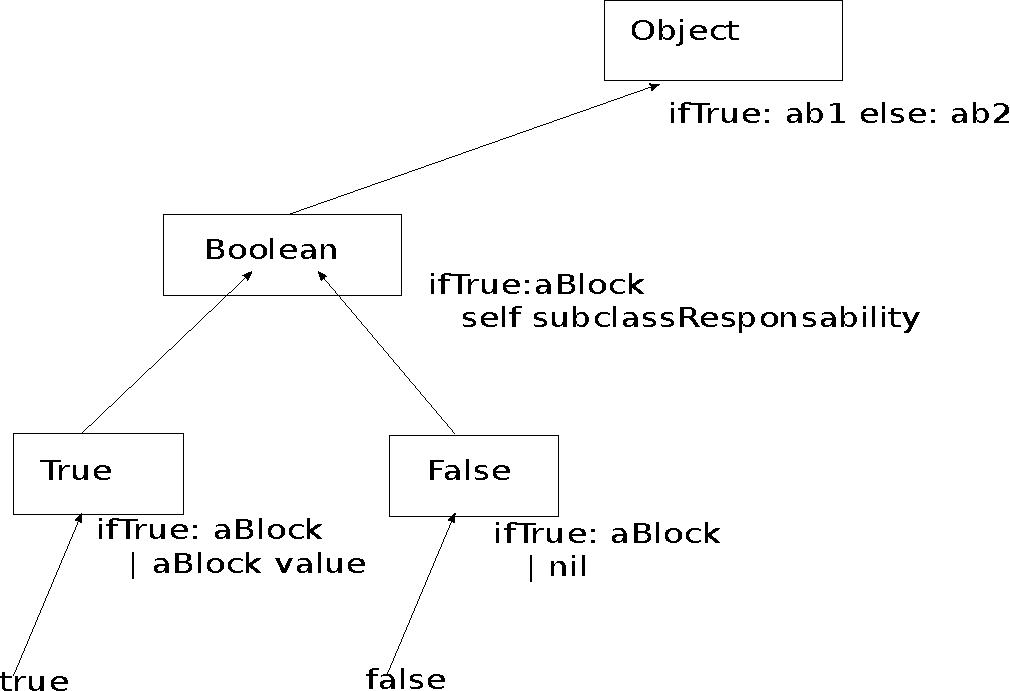
\includegraphics[width=180px]{Images/fig1.pdf}

\titre{Plan de cours}
\begin{enumerate}
	\item Introduction
	\item Concepts de base (objet, classe, envoi de message, hiérarchie)
	\item Illustrations et exemples (Java, Simula, SmallTalk
	\item Etude comparative de LO
	\item TP (Java, Eclipse)
\end{enumerate}

\titre{Histoire d'Ada}
Le département de la défense américain (Dod) est : 
\begin{itemize}
	\item Plus gros consommateur de logiciels
	\item 1968 - 73 : Le coût des SI augmente et le coût du matériel chute
	\item 73 : 7,5 milliards de dollars pour les Si
	\item 75 : 450 langages différents
	\item Réutilisabilité et partage de code inexistants
	\item 1983 : naissance d'Ada en réponse à la crise du logiciel et pour résoudre les pbs liés au dev de gros logiciels
	\item non issu d'un projet académique ou de recherche interne
\end{itemize}
Idée : Un seul langage incorporant tous les bons concepts de GL.\\

\titre{Paradigmes de programmation}
\begin{itemize}
	\item impérative
	\item fonctionnelle
	\item logique
	\item objet
	\item par contraintes
\end{itemize}

\newpage

\titre{Les domaines révolutionnés par la POO}
\begin{itemize}
	\item Génie logiciel (analyse, conception, programmation)
	\item Bases de données
	\item Intelligence artificielle (représentation des connaissances, programmation par agents)
\end{itemize}

\titre{Quel objet ?}
\begin{itemize}
	\item Des problématiques différentes $\rightarrow$ Des approches objet différentes
	\item Une préoccupation commune (approche modulaire de la complexité)
\end{itemize}
Pour distinguer les approches différentes, on change le voc :
\begin{itemize}
	\item Génie Logiciel : Objet
	\item IA : Schéma
	\item Ingénierie collaborative : Agent
	\item Bases de données : RDF
\end{itemize}

\titre{Quels languages :}
\begin{itemize}
	\item Java sous éclipse principalement
	\item Simula
	\item SmallTalk
\end{itemize}
